\chapter{Konzepte \& Architektur}
\label{ch:konzepte_architektur}
\section{Konzepte}
Für die Bewältigung der Anforderungen an die Softwarelösung wurden einige Konzepte entwickelt, welche Einfluss auf die einzelnen Komponenten und die Architektur genommen haben. Die Softwarelösung soll wie unter \ref{ch:anforderungen_section} \nameref{ch:anforderungen_section} beschrieben, die Möglichkeit bieten eine Karte darzustellen, auf welcher die Simulationsdaten dargestellt werden und bearbeitet werden können. Die Bearbeitung sollte jedoch keinen Einfluss auf die Stammdaten haben. Diese Konzepte werden in den folgenden Kapiteln beschrieben.\\
TODO
Um die Anforderungen (siehe. \ref{ch:anforderungen_section}) an die Softwarelösung zu bewältigen, wurden Konzepte für die einzelnen Komponenten entwickelt, welche Einfluss auf die Architektur haben.
\subsection{Datentiles}
\label{ch:datentiles}
Um die grosse Datenmenge (ca. 2,8 Millionen Datensätze für die Schweiz) zu bewältigen, wurde ein bewährtes Verfahren für Kartendarstellung verwendet. Dabei werden die Daten nicht als gesamtes geliefert, sondern über Tiles angefragt. Ein Tile ist ein Quadrat, welches ein vordefinierten Bereich der Welt deckt. Durch die Anforderung eines dieser Quadrate kann sichergestellt werden, dass nicht zu viele Daten auf einmal angefragt werden. Ein weiteres Konzept in Verbindung mit diesem wird unter \ref{sec:concept_preprocessing} \nameref{sec:concept_preprocessing} beschrieben. Dabei werden die Daten für jede Zoomstufe bewertet und nur ausgegeben, wenn diese Relevant sind. Durch dieses Konzept kann die Datenmenge, die von der Website verarbeitet werden muss, stark reduziert werden.
\begin{figure}[H]
\centering
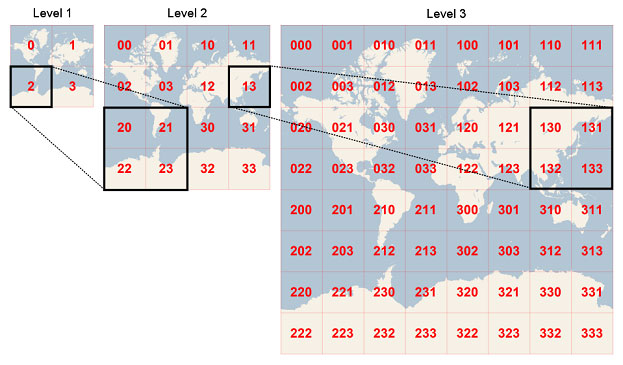
\includegraphics[height=7cm]{images/BingMapsTileSystem.jpg}
\\Quelle: \href{https://msdn.microsoft.com/en-us/library/bb259689.aspx}{https://msdn.microsoft.com/en-us/library/bb259689.aspx}
\caption{Fixe Aufteilung der Welt in Tiles und Berechnung des QuadKey}
\label{fig:tilesystem}
\end{figure}
\noindent
Um von einem Eintrag auf das Tile zu schliessen, in welchem dieser sichtbar ist, wird ein Schlüssel (QuadKey) berechnet. Der QuadKey benennt eindeutig das kleinstmögliche Tile in welchem der ganze Eintrag (z.B. eine Strasse) angezeigt werden kann. Der QuadKey wird nach dem System in Abbildung \ref{fig:tilesystem} erstellt. Dabei wird auf der äussersten Zoomstufe die Welt in 4 Tiles aufgeteilt. Diese werden nummeriert. z.B. 0 für links oben, 1 für rechts oben. Um die nächste Stufe der Tiles zu erstellen, wird jedes Tile wieder in 4 Tiles aufgeteilt und dann ebenfalls nummeriert. Dabei wird als Prefix die Nummer des alten Tiles verwendet. Dadurch kann jedes Tile auf jeder Zoomstufe eindeutig adressiert werden. Der QuadKey bietet auch die Möglichkeit, mit Hilfe des Prefix alle Tiles unterhalb eines Tiles zu berechnen. So starten alle QuadKeys, welche auf einer beliebigen Zoomstufe in einem Tile unterhalb des linken oberen Tile auf Level 1 sind, mit einer 0. Dieser Ansatz kann für die Filterung der Daten verwendet werden.
\subsection{Preprocessing und Bewertung der Daten}\label{sec:concept_preprocessing}
Um die Zugriffszeiten der Datenbank zu erhöhen, werden die Daten beim Importieren vorberechnet. Durch diesen Vorgang werden bewusst Redundanzen in das Datenmodell eingeführt. Diese Redundanzen erlauben den Zugriff auf Daten ohne teure JOIN Statements oder SQL-Funktionen aufzurufen. Auf die Vorberechnungen, welche im Datenmodell verwendet werden, wird tiefer im Abschnitt \ref{sec:tilingdataimplementation} \nameref{sec:tilingdataimplementation} eingegangen. Um weiteren Berechnungsaufwand zu reduzieren, wird jeder Datensatz neben der Vorberechnung auf seine Anzeigewichtigkeit bewertet. Dabei wird berechnet, ab welcher Stufe z.B. die Strasse dargestellt wird.

\subsection{Changeset}
Um Daten der User abzuspeichern wurde ein Konzept entwickelt, mit welchem erreicht werden soll, dass Daten gespeichert werden können ohne die Stammdaten anzupassen. Wenn für jeden User die Stammdaten kopiert werden müssten, würde das zu einer unnötigen Vergrösserung der Datenmenge führen. Dadurch wurde das Changeset Konzept entwickelt. Changesets erlauben es, Änderungen aufzuteilen und nur die Differenz zu den Stammdaten abzulegen. Dadurch wird es ermöglicht die Zugriffszeiten auf die Stammdaten konstant zu halten. Das Changeset ist als Abbild der Stammdaten aufgebaut. Dabei werden jedoch nur Felder gespeichert, welche sich zu den Stammdaten unterscheiden. Da ein Changeset nicht direkt Stammdaten enthält werden Änderungen an den Stammdaten übernommen, so fern sie nicht durch das Changeset bearbeitet wurden.
\subsection{UI-Konzept}
Das Ziel für den Verkehrsmodell-Fallstudien Editor ist es, dass Tool dem Kunden übergeben zu können und dann die von Ihm erstellen Aufträge zu simulieren. Ebenfalls sollten Mitarbeiter von Senozon die Softwarelösung ohne grosse Einarbeitungszeit verstehen können. Um diesen Anforderungen zu entsprechen, musste die Benutzeroberfläche möglichst intuitiv konzeptioniert und implementiert werden. Als Inspirationsquelle für das User Handling wurde Google Maps \cite{GoogleMaps}, sowie der ID Editor \citep{IDEditor} von OpenstreetMap verwendet.
\newpage
\subsubsection{Google Maps}
Google Maps ist eines der weit verbreitetsten Kartensysteme. Dadurch sind sich die User an das Handling von Google Maps gewöhnt und Systeme mit ähnlichen Aufbau sind intuitiv. Die Vorteile des System von Google Map ist die intuitive Bedienung, gekoppelt an ein einfaches, aufgeräumtes und leichten Design.
\begin{figure}[H]
\centering
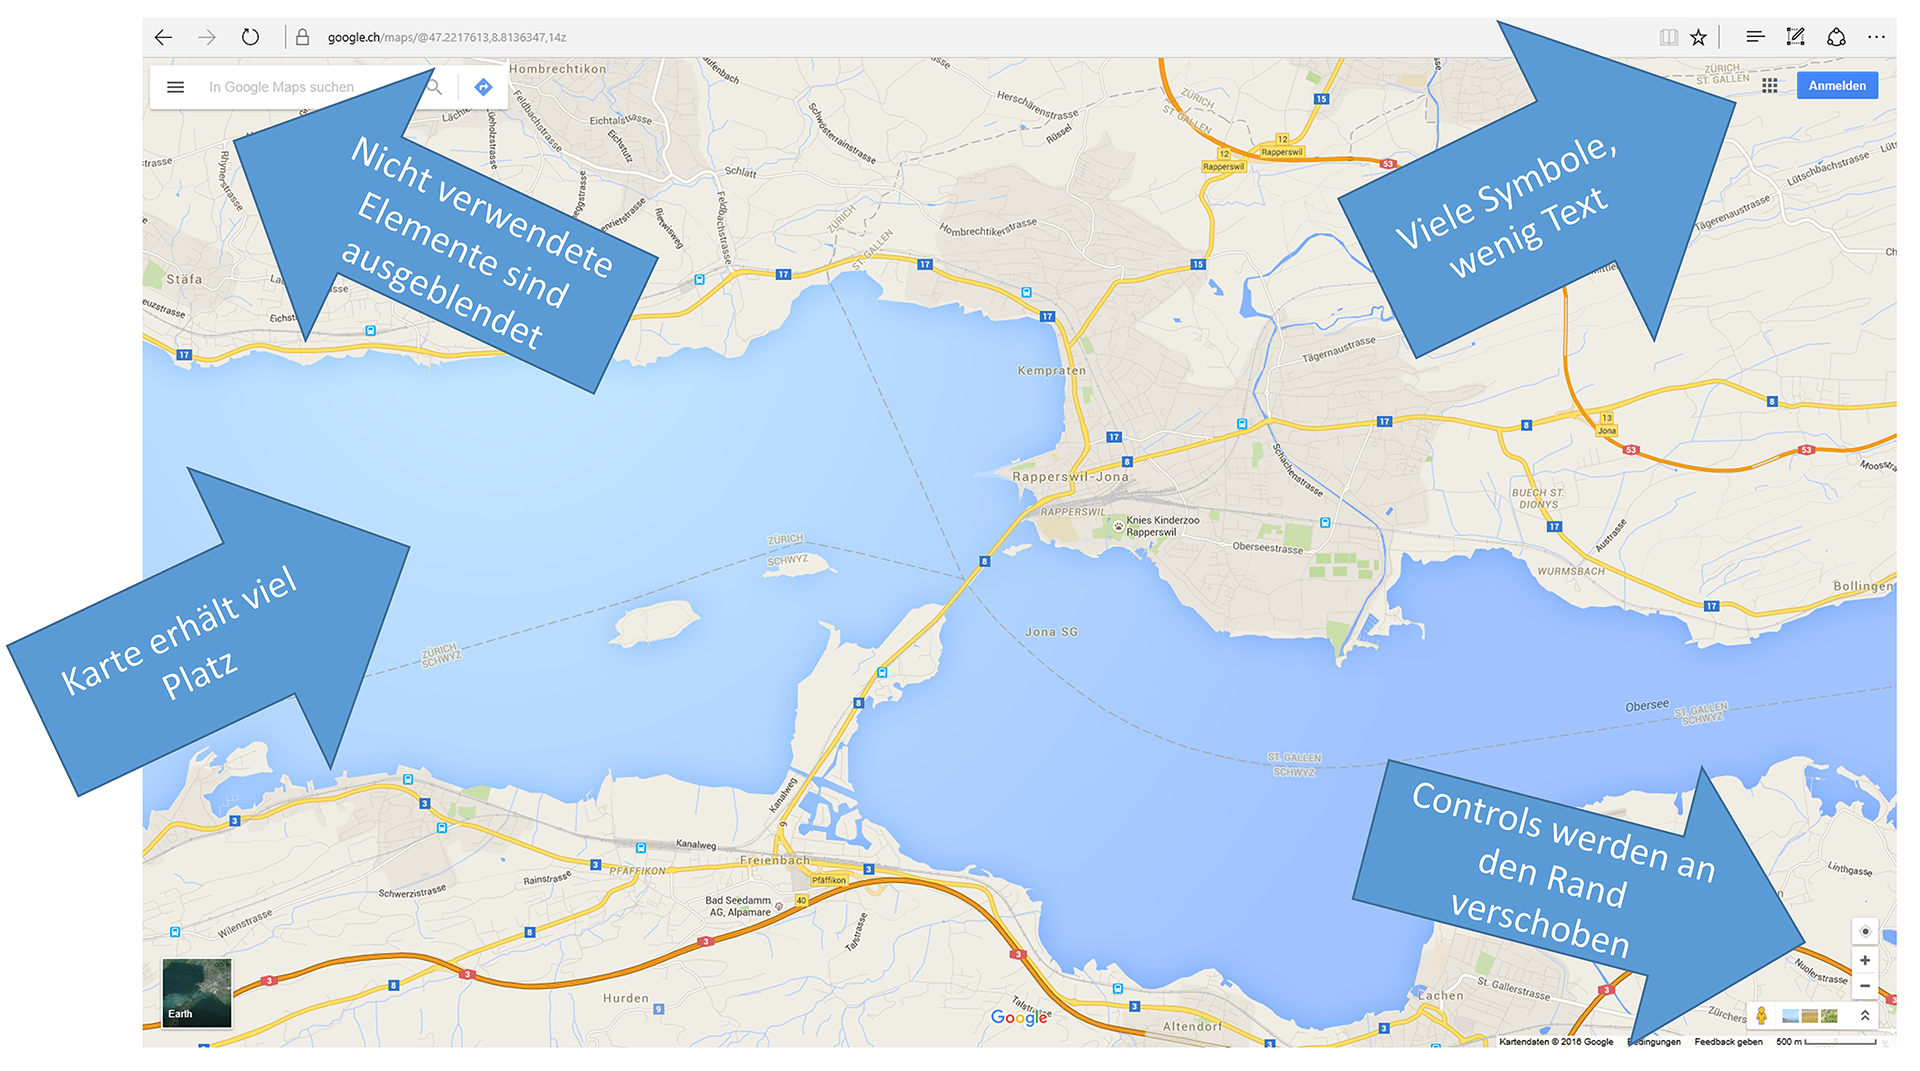
\includegraphics[height=7cm]{images/AnalyseGoogle.png}
\caption{Analyse Google Maps}
\label{fig:googlemaps}
\end{figure}
\noindent
Die Abbildung \ref{fig:googlemaps} \nameref{fig:googlemaps} zeigt die Analyse von Google Maps. Die Karte bei Google Maps erhält sehr viel Platz und alle Controls werden um den Hauptbereich der Karte herum angeordnet. Dadurch wird der User nicht von der Kernaufgabe der Seite abgelenkt. Bei kleineren Karten fühlt sich der User schneller eingegrenzt muss mehr aufwand in Scrolling investieren, was stören kann. Das User Interface passt sich laufend an die Nutzung des Users an. Wenn der User also fertig ist, ein Ort zu finden und eine Route berechnen will, wird das Menü für die Route seitlich eingeblendet. Dadurch wird der Karte Platz weggenommen, welcher jedoch nicht mehr benötigt wird, da der User eine Route berechnen will. Um Platz für die Controls zu sparen, werden viele Symbole anstatt Text eingesetzt.
\subsubsection*{Ergebnisse Analyse}
Die Analyse von Google Maps ergab folgende Punkte, welche in das Design des Verkehrsmodell-Fallstudien Editor einfliessen sollen:
\begin{itemize}
\item Der Karte viel Platz einräumen.
\item Menüs, welche nicht dem aktuellen Use Case entsprechen, ausblenden.
\item Viele Symbole, wenig Text.
\end{itemize}
\section{Architektur}
\begin{figure}[H]
\centering
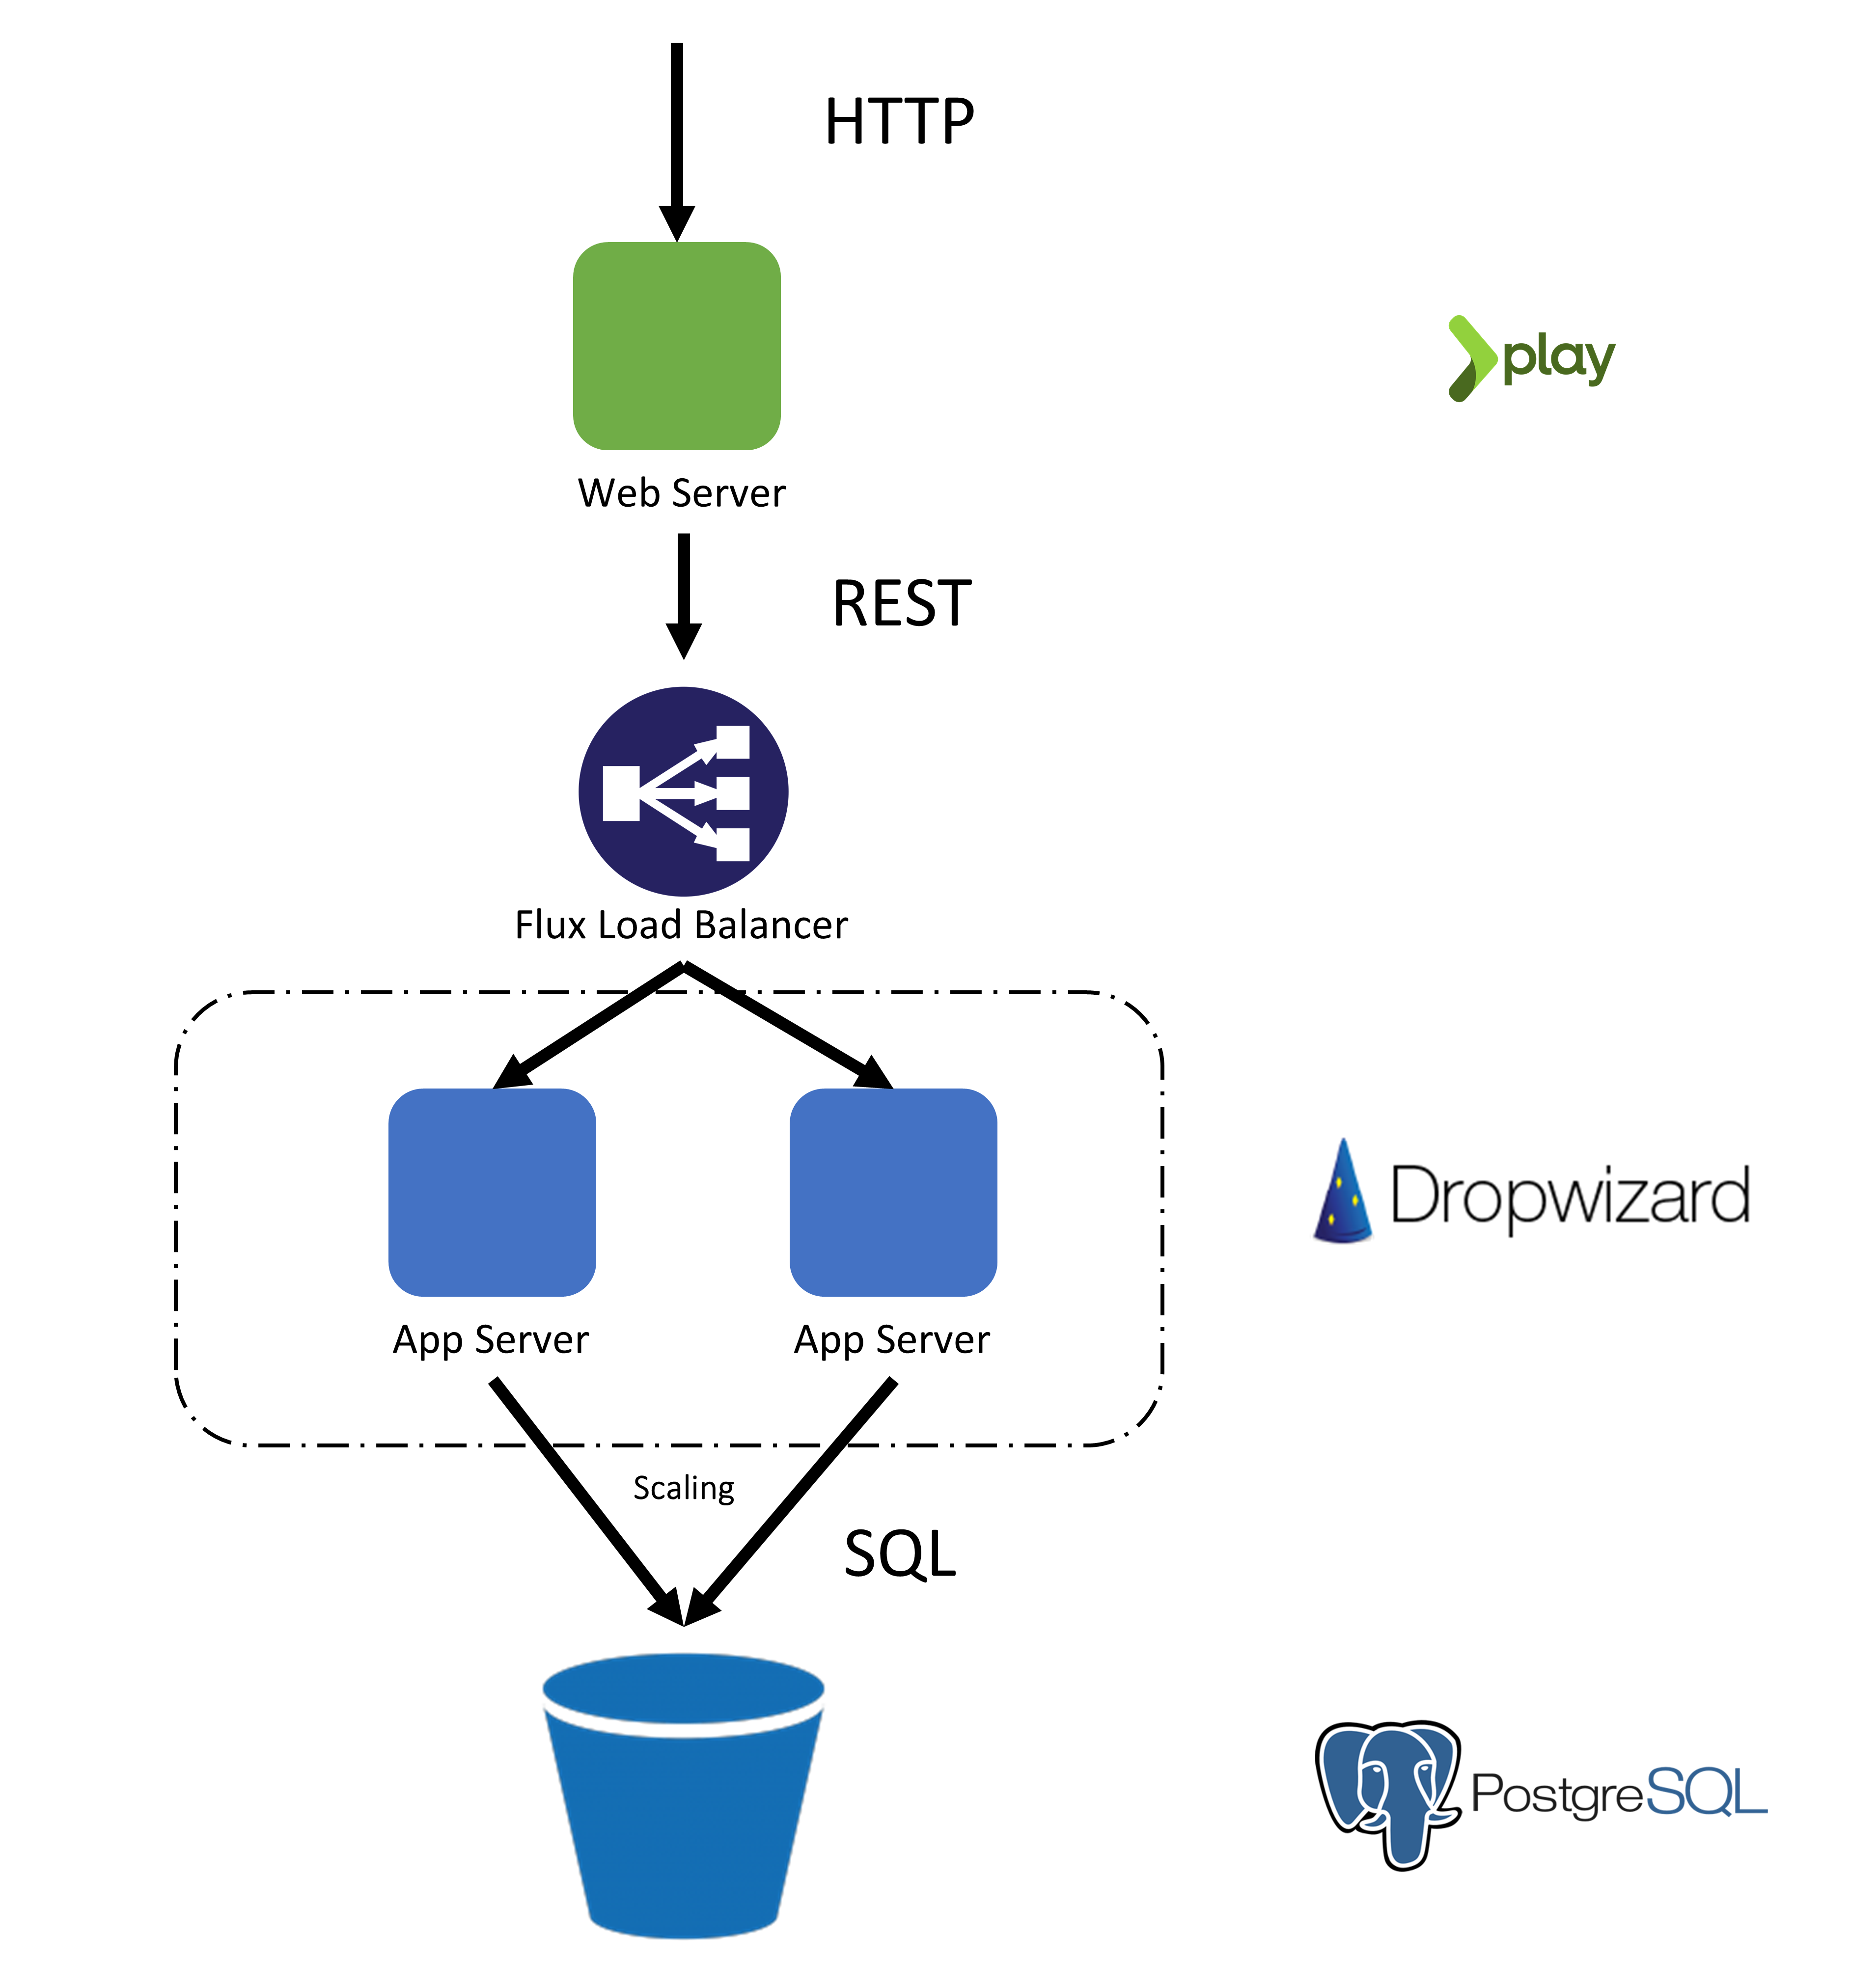
\includegraphics[height=10cm]{images/Architektur.png}
\caption{Tier des Verkehrsmodell-Fallstudien-Editor}
\label{tier_architecture}
\end{figure}
Durch die Anforderungen bezüglich Performance und Antwortgeschwindigkeiten musste die Architektur für die Softwarelösung des Verkehrsmodell-Fallstudien-Editor skalierbar aufgebaut werden. Eine Entkopplung der Komponenten erlaubt eine Verteilung und kann daher die Last auf dem einzelnen Server senken. Die Softwarelösung für den Verkehrsmodell-Fallstudien-Editor ist daher als 3-Tier Applikation aufgebaut. Der Frontside-Tier ist ein Webprojekt implementiert mit dem Play Framework. Der Backend-Tier wird als REST Service (Maturity Level 2) mit Dropwizard entwickelt. Der Daten-Tier wird durch eine PostgreSQL Datenbank bereitgestellt. Der Backend-Tier wird durch eine Load Balancer skalierbar und kann daher mehrere Anfragen parallel ausführen.\\
\begin{figure}[H]
\centering
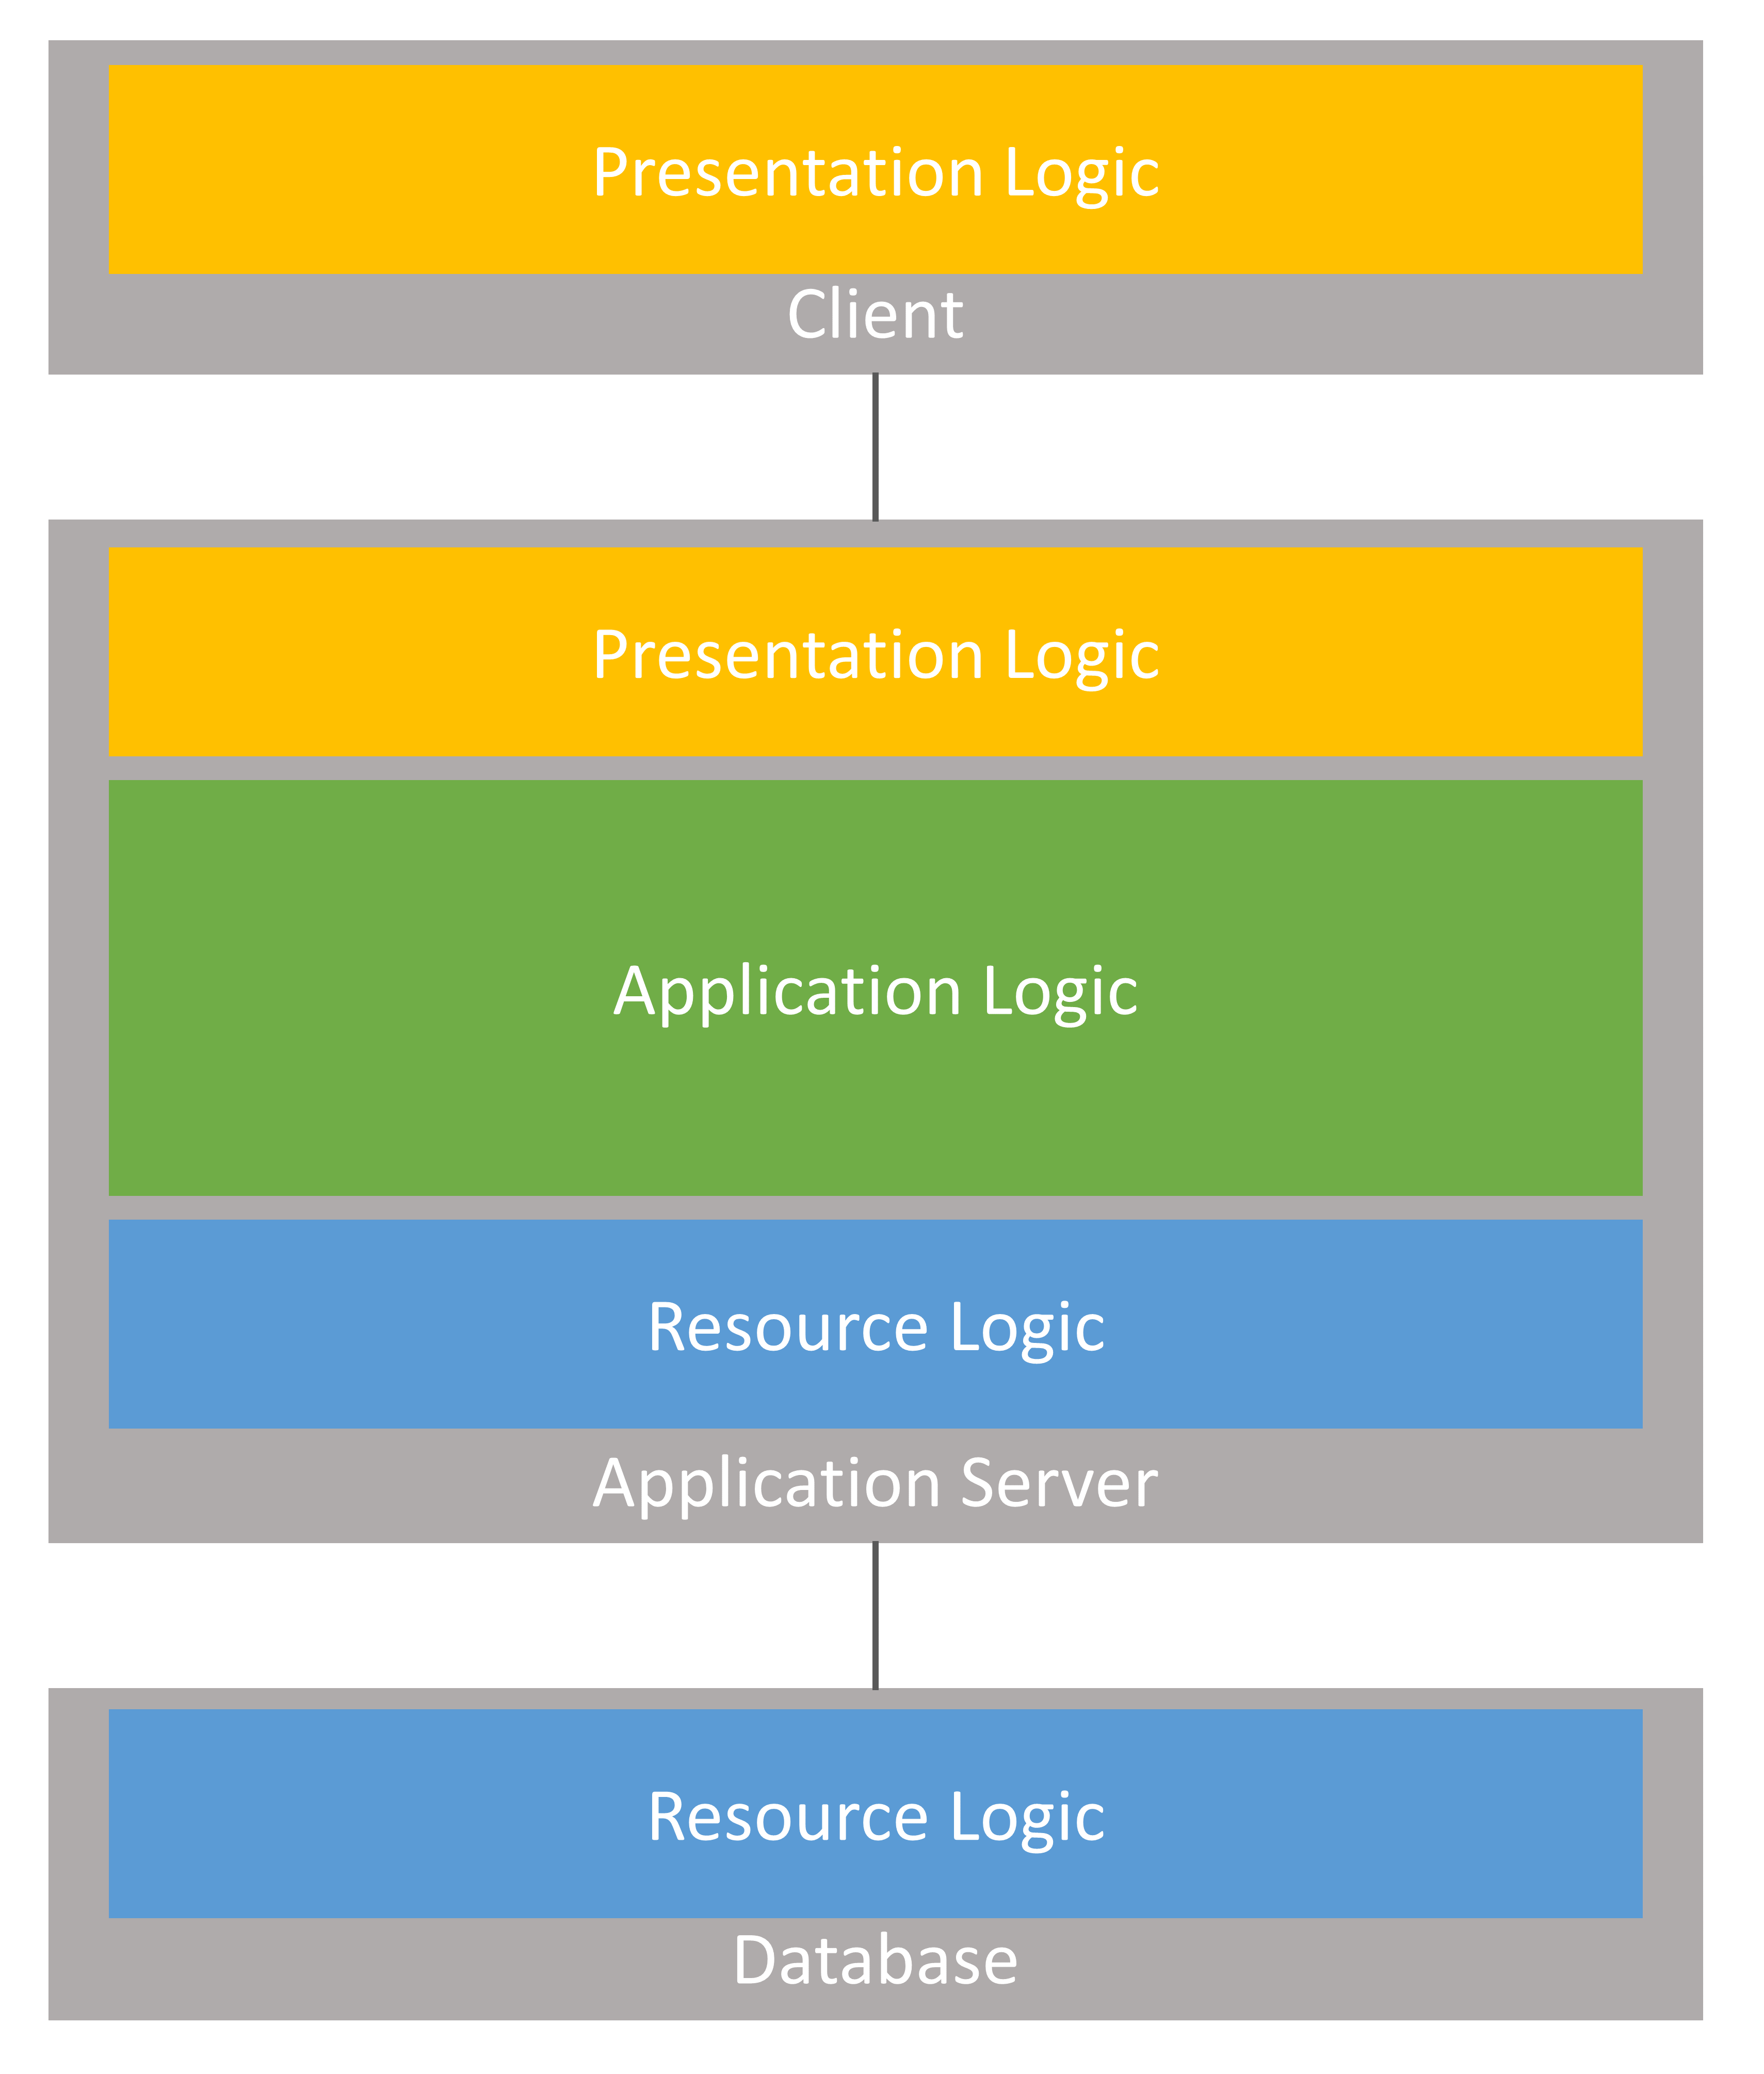
\includegraphics[height=10cm]{images/layers.png}
\caption{Tier- / Layeraufteilung}
\label{fig:tierlayers}
\end{figure}
\noindent
Die Aufteilung der Presentation Logic auf den Client-Tier, sowie den Backend-Tier erlaubt es die Last der Datendarstellung auf die verschiedenen Komponenten zu verteilen. Die Vorbereitung und Aufbereitung der Daten wird vom Backend-Tier vorgenommen. Die Daten werden im für den Client lesbaren Format übertragen. Das Rendering der Daten übernimmt dann der Client, was dazu führt, dass der Server bei diesen Aufgaben entlastet wird.
\newpage
\section{SimMap-Editor}
\begin{figure}[H]
\centering

\includegraphics[height=2cm]{images/presentationlayer.png}
\caption{SimMap-Editor}
\label{fig:presentationlayer}
\end{figure}
\noindent
Der SimMap-Editor ist die Frontend-Komponente der Architektur und basiert auf dem Play Framework. Der Client Tier ist eine in Javascript entwickelte Software, welche auf den Backend-Tier zugreift, um die Daten auf der Karte darzustellen. Dabei übernimmt der Client-Tier das Rendering der Daten.
\section{SimMap-Service}
TODO
\section{Datenbank}
TODO